\chapter{Finding appropriate hyperparameters for training}


\section{Reward functions capability check}

Previous sections introduced the composite reward function. The composite reward function consists of a weighted sum of individual reward functions. The individual reward functions are designed to encourage the agent to learn the desired behaviour. The goal is to achieve an agent that completes the parcour without collisions, this is encapsulated in the event reward function. However the event reward function is a very sparse signal, which makes it hard for the agent to learn from. The other individual reward functions are designed to be dense reward functions, they give rewards in every episode step.

It is important to find appropriate weights of the individual reward functions for the composite reward function. We are conducting experiments to analyse the usefullness of the individual reward functions. First we analyse if the agent is capable of learning the behaviour encouraged by the reward function.
This is done by training the agent with only one reward function at a time. The reward function's coefficient is set to one. The coefficients of the other reward functions are set to zero. The agent is trained on easy tracks with a Random spawnOrientation and standard lightSetting to reduce the difficulty of learning the encouraged behaviour.


The experiment results are shown in \ref{table:reward_functions_behaviour}. The agent is capable of learning the behaviour encouraged by the distanceReward and velocityReward functions. However the agent is not capable of learning the behaviour encouraged by the eventReward and orientationReward functions. 

% TODO nochmal ausführen und dokumentieren oder ist das schon in Excel?

\begin{table}
\begin{center}
\begin{tabular}{|| c | p{0.3\textwidth} | p{0.3\textwidth} | p{0.1\textwidth} ||} 
    \hline
    function name & encouraged behaviour & learned behaviour  & expected behaviour learned? \\ [0.5ex] 
    \hline\hline
    eventReward &  agent drives through the parcour without collisions & agent turns on the spot continuously & no \\ 
    \hline
    distanceReward & agent drives towards the next goal & agent drives towards the next goal & yes \\
    \hline
    orientationReward & agent turns towards closest goal & agent turns around on the spot continuously & no \\
    \hline
    velocityReward  & full speed ahead (no turning) & full speed ahead (no turning) & yes \\
    \hline
\end{tabular}
\end{center}
\caption{Agent capability check for individual reward functions.}
\label{table:reward_functions_behaviour}
\end{table}


\section{Chosen Reward function}

As a result of the capability check, the distanceReward function was determined to be most suitable for the training process. Further tests of combining the distanceReward with the eventReward function were carried out. The goal was to find a parameters for the composite reward function that would allow the agent to learn to complete the tracks without collisions. The distanceReward function alone does not penalize collisions as heavily as the eventReward. 
Experiments were executed using both functions together with different coefficients. The behaviour of the agent and the obtained rewards were monitored during training. The results showed that the agent was not capable of leaning from the combined rewards, regardless of the combinations of coefficients.

The distanceReward showed the best results when used alone. The agent was able to learn the desired behaviour and complete the tracks reliably. The distanceReward function was chosen as the only reward function for the final training process. The other reward functions function were not used in the training process. 
The coefficient for the distanceReward was set to 1, the others were set to 0. As a result the total reward function is defined as \ref{fig:final_reward_function}. 

\begin{figure}
    \centering
    \begin{align*}
         R(s_t,a_t) &= \Delta distance(Agent, NextGoalPosition) \cdot \Delta T \nonumber \\
    \end{align*}
    \caption{Final reward function}
    \begin{tabular}{r@{: }l r@{: }l}
    $s_t$& state t & $a_t$& action in state t 
    \end{tabular}
    \label{fig:final_reward_function}
\end{figure}


\section{Experiments mixed difficulty setting}
\label{cha:experiment_mixed_difficulty}

In the experimentation pahse of this project the agents were trained exclusively on tracks of a specific difficulty setting. This was done to analyse the capability of the jetbot agent and to find appropriate hyperparameters that allow the agents to learn. These hyperparameters include the agent camera image dimensions, the $fixedTimestepLength$, the amount of steps to collect in each iteration and more. 
The experiments showed that it is possible to train the agent with the right hyperparameters to solve tracks of a particular difficulty level when the agent is exclusively trained on that difficulty level. For example the agent could be trained to solve the medium tracks very successfully without needing to encounter easy tracks during training. The light settings were restricted to standard during this experimentation to focus on the difficulty levels.

The experiments produced a set of hyperparameters that could be used for training the agent on the different difficulty levels exclusively. Further evaluation of these agents showed that they were able to generalize to the tracks of lower difficulty levels. For example the agent that was only trained on hard tracks with standard light conditions could solve the easy and medium tracks as well.

The next step was to train the agent on all difficulty levels at the same time. The goal was to find hyperparameters that would allow the agent to learn to solve all difficulty levels better than with the previous exclusive training. The agent was trained on all difficulty levels at the same time with the same hyperparameters that were used before. The $trainingMapType$ parameter was set to $randomEval$, this results in split of 20\% easy, 40\% medium and 40\% hard tracks.

The training with mixed tracks for the data collection episodes failed. The agent was not able to learn to solve the tracks as successfully as the isolated training. Further changes to the hyperparameters did not improve the learning process. For example the amount of data collected in each iteration was increased to balance out the increased variety of tracks.

% put a figure here? or in the appendix?

\section{Experiment mixed light setting hyperparameter}
\label{cha:experiment_mixed_light}

Experiment mixed training hyperparameter

explain how the training with mixed light setting was worse than the training with fixed standard light setting

\subsection{current training run}
currently training is running to check if the training with mixed light settings works if it is only run on hard tracks
does this improve?


\section{Most successful policy}

This section describes how the most successful policy was implemented and trained. This policy is used for the evaluations of the three main research goals.
The policy was configured to use the three preprocessing steps downsampling, greyscaling and histogram equalization. The policy used a frame stacking of 10. The agent camera image had a resolution of $500x168$ which was downsampled to $250x84$. This results in an observation space of shape $[84, 250, 10]$. The duration of steps was fixed to $0.3$ seconds.
The neural network follows the earlier descriptions exactly \ref{sec:network_architecture}. It consisted of a feature extractor part with 3 convolutional layers and one fully connected layer. The feature extractor takes the observation as input, its outputs are used by the action and value head. The action and value head each consist of a single fully connected layer. The entire network is trained together end-to-end using backpropagation of the loss defined by the PPO algorithm.

The policy was trained exclusively using the distance reward. The other reward functions were not used \ref{fig:final_reward_function}.

The episodes for data collection used the standard light setting and difficult tracks only. The agent was initialized with random orientations. The episodes were not reset upon collision.
The training was configured to use 10 environments in parallel to collect data. 2560 samples were collected in each data collection step. The training was terminated after a total of 6500000 steps. 32700 full episodes were executed to collect these samples. 2540 data collection and model training iterations were executed in total. The total training duration was 3.23 days.
The training progress over the three days can be seen in figure \ref{fig:training_most_successful_model}. The model reached a success rate of 100\% for the collected episodes.

The full training config can be found in the appendix \ref{cha:most_successful_config}.

\begin{figure}
    \centering
    \subfigure[Distance Reward]{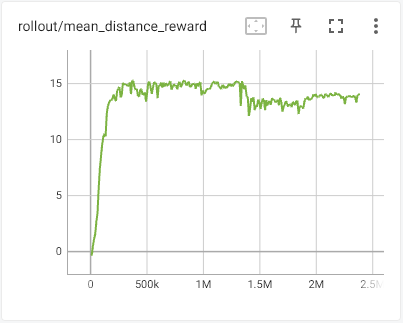
\includegraphics[width=0.3\textwidth]{Bilder/tensorboard_images/successfulTraining_distance_reward.png}}
    \subfigure[Goal completion rate]{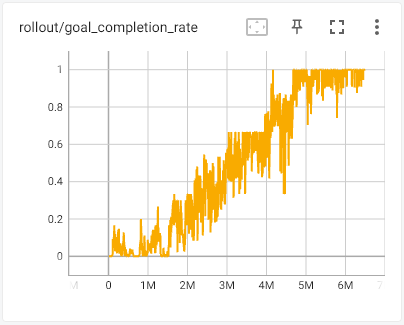
\includegraphics[width=0.3\textwidth]{Bilder/tensorboard_images/successfulTraining_goal_completion_rate.png}}
    \subfigure[Success rate]{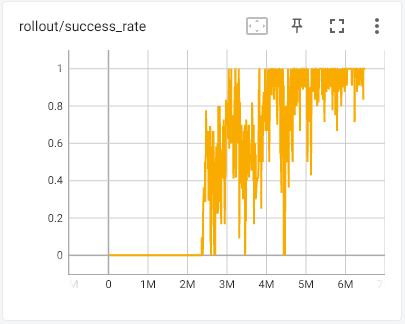
\includegraphics[width=0.3\textwidth]{Bilder/tensorboard_images/successfulTraining_success_rate.png}}
    \caption{Properties of the collected episodes over time for the most successful model}
    \label{fig:training_most_successful_model}
\end{figure}